%%%%%%%%%%%%%%%%%%%%%%%%%%%%%%%%%%%%%%%%
\subsection{VPC: Pipelined-RAM 一致性验证}

\newcommand{\pram}{Pipelined-RAM}
\newcommand{\PRAM}{PRAM}
\newcommand{\vpc}[1]{\ifthenelse{\isempty{#1}{}}{\textsf{VPC}}{\textsf{VPC-\MakeUppercase{#1}}}} 
\newcommand{\npc}{$\sf{NP}$-complete}
\newcommand{\npcn}{$\sf{NP}$-completeness}
\newcommand{\rwclosure}{\textsc{RW-Closure}}
\newcommand{\readcentric}{\textsc{Read-Centric}}
%%%%%%%%%%%%%%%
\begin{frame}{VPC 工作在技术框架中的位置}
  \fig{width = 0.50\textwidth}{figures/3d-framework-vpc.pdf}{VPC --- \pram{} {\small (\PRAM{})} 一致性验证.}
\end{frame}
%%%%%%%%%%%%%%%
\begin{frame}{研究动机}
  \question{问题: 为什么要验证 \PRAM{} 一致性?}
  \vspace{0.10cm}

  \begin{description}
    \setlength{\itemsep}{10pt}
	\item[验证:] 测试/确认系统是否提供了其所声称的数据一致性 
	  \citeinbeamer{Amazon}{SOSP}{07} \citeinbeamer{Golab}{PODC}{11}
	\pause
	\item[PRAM:] 包含存储系统常提供的``会话''一致性\\
	  \citeinbeamer{Terry}{PDIS}{94} \citeinbeamer{Brzezi$\acute{\text{n}}$ski}{PDP}{04}
  \end{description}

  \pause
  \fig{width = 0.50\textwidth}{figures/pram-monotonic-writes-example.pdf}{\PRAM{} 保证``单调写''性质 \citeinbeamer{Terry}{PDIS}{94} \citeinbeamer{Brzezi$\acute{\text{n}}$ski}{PDP}{04}.}
\end{frame}
%%%%%%%%%%%%%%%
\begin{frame}{VPC 问题定义}
  \begin{cdef}[VPC: Verifying PRAM Consistency]
    VPC 判定问题:
	\vspace{8pt}
    \begin{description}
	  \setlength{\itemsep}{8pt}
      \item[实例:] 系统执行 {\small (execution $e$)}
      \item[问题:] 该执行 $e$ 是否满足 PRAM 一致性模型 {\small ($\mathcal{C}$)}? 
		\[
		  e \in \mathcal{C} \Rightarrow \set{0,1}?
		\]
    \end{description}    
  \end{cdef}
\end{frame}
%%%%%%%%%%%%%%%
\begin{frame}{VPC 问题定义}
  \begin{cdef}[系统执行]
	系统执行 ($e$) $\triangleq$ $\{h_p \mid h_p: \text{进程 } \;p \text{ 上的读写操作序列}\}$

	\vspace{0.30cm}
	\textcolor{blue}{规模 $n$:} 系统执行中操作的总数
  \end{cdef}

  \fignocaption{width = 0.50\textwidth}{figures/execution-example.pdf}
\end{frame}
%%%%%%%%%%%%%%%
\begin{frame}{VPC 问题定义}
  \begin{cdef}[\PRAM{} 一致性模型]
	\begin{center}
	  系统执行 $e$ 满足 \PRAM{} 一致性 \\
	  $\iff$\\
	  $\forall p:$ $p$ 上\textcolor{blue}{所有操作}与其它进程上所有\textcolor{blue}{写操作}存在\textcolor{red}{合法}调度.
	\end{center}
  \end{cdef}

  \fignocaption{width = 0.50\textwidth}{figures/execution-example.pdf}

  \pause
  \vspace{-0.80cm}

  \begin{gather*}
	p_{0}: Wf2\; Wf1\; Wz2\; Wz1\; Wy2\; Wy1\; \textcolor{brown}{Rf1} 
	Wx5\; Wx3\; Wx2\; Wc1\; \textcolor{brown}{Rc1} \\
	\textcolor{brown}{Rz1} \textcolor{brown}{Ry1}
	Wa1\; \textcolor{brown}{Ra1} Wb1\; \textcolor{brown}{Rb1} \textcolor{brown}{Rx2}
  \end{gather*}
\end{frame}
%%%%%%%%%%%%%%%
\begin{frame}{VPC 问题分类}
  \begin{table}[!t]
    \centering
	\caption{VPC 问题的四种变体 (按``执行''的类型) 及复杂度分析 ($\textcolor{red}{[\ast]}$\textcolor{red}{: 本文工作}).}
	\renewcommand\arraystretch{1.2}
    \begin{tabular}{|c|c|c|}
      \hline
      & \it (S)ingle variable  & \it (M)ultiple variables
      \\ \hline
	  {\it write (D)uplicate values} &
	  \innercell{c}{VPC-SD \\ \uncover<2->{\textcolor{red}{\small (\npc{}) $[\ast]$}}} &
	  \innercell{c}{VPC-MD \\ \uncover<2->{\textcolor{red}{\small (\npc{}) $[\ast]$}}}
      \\ \hline
	  \only<1-2>{\it write (U)nique value}\only<3>{\cellcolor{brown!80}{\it write (U)nique value}} &
	  \innercell{c}{VPC-SU \\ \uncover<2->{\textcolor{blue}{\small (P) \citeinbeamer{Golab}{PODC}{11}}}} &
	  \innercell{c}{VPC-MU \\ \uncover<2->{\textcolor{red}{\small (P) $[\ast]$}}}
      \\ \hline
    \end{tabular}
  \end{table}

  \vspace{10pt}
  
  \uncover<3->{\textcolor{brown}{\centerline{Read-mapping \citeinbeamer{Gibbons}{SICOMP}{97}: $\forall r, \exists! w, f(r) = w$.}}}
\end{frame}
%%%%%%%%%%%%%%%
\begin{frame}{VPC-SD (VPC-MD) 是 \npc{} 问题}
  多项式规约: 从 \textsc{Unary 3-Partition} 到 \vpc{sd}.

  \fig{width = 0.40\textwidth}{figures/vpcsd-npc.pdf}{对应于 \textsc{Unary 3-Partition} 实例 $A = \{2,2,1,1,1,1\}, m = 2, B = 4$ 的 VPC 执行.} 
\end{frame}
%%%%%%%%%%%%%%%
\begin{frame}{VPC-MU 的多项式算法 \rwclosure{}}
  \begin{figure}[h!]
    \centering
    \begin{adjustbox}{max totalsize = {0.60\textwidth}{1.00\textheight}, center}
	  % http://tex.stackexchange.com/questions/54794/using-a-pgfplots-style-legend-in-a-plain-old-tikzpicture#54834

% argument #1: any options
\newenvironment{customlegend}[1][]{%
    \begingroup
    % inits/clears the lists (which might be populated from previous
    % axes):
    \csname pgfplots@init@cleared@structures\endcsname
    \pgfplotsset{#1}%
}{%
    % draws the legend:
    \csname pgfplots@createlegend\endcsname
    \endgroup
}%

% makes \addlegendimage available (typically only available within an
% axis environment):
\def\addlegendimage{\csname pgfplots@addlegendimage\endcsname}

%%--------------------------------

% definition to insert numbers
\pgfkeys{/pgfplots/number in legend/.style={%
        /pgfplots/legend image code/.code={%
            \node at (0.295,-0.0225){#1};
        },%
    },
}
%%%%%%%%%%%%% For Legend %%%%%%%%%%%%%%%%%%%%%%

\begin{tikzpicture}[read/.style = {fill = orange, font = \Large}, 
write/.style = {fill = lightgray, font = \Large},
on grid, every node/.style = {node distance = 1.0cm and 1.6cm}, 
po/.style = {->, very thick, blue}]
%   	      \draw[step = {(1.5,1)}, style=help lines] (-1.5,0) grid (10.5,4);
	% process 0
	\begin{scope}[yshift = 4.0cm]
		\node (wy1) [write] at (0,0) {$Wy1$};
		\node (rf1) [read, right = of wy1] {$Rf1$};
		\node (rc1) [read, right = of rf1] {$Rc1$};
		\node (rz1) [read, right = of rc1] {$Rz1$};
		\node (ry1) [read, right = of rz1] {$Ry1$};
		\node (ra1) [read, right = of ry1] {$Ra1$};
		\node (rb1) [read, right = of ra1] {$Rb1$};
		\node (rx2) [read, right = of rb1] {$Rx2$};
	\end{scope}

	% process 1
	\begin{scope}
		\node (wf1) [write, node distance = 1.5cm, below = of rf1] {$Wf1$};
		\node (wx2) [write, node distance = 1.5cm and 3.0cm, below left = of rx2] {$Wx2$};
		\node (wc1) [write, node distance = 3.0cm, right = of wx2] {$Wc1$};
	\end{scope}

	% process 2
	\begin{scope}[]
		\node (wa1) [write, node distance = 3.0cm and 3.5cm, below left = of ra1] {$Wa1$};
		\node (wx3) [write, left = of wa1] {$Wx3$};
		\node (wz2) [write, left = of wx3] {$Wz2$};
		\node (wf2) [write, left = of wz2] {$Wf2$};
	\end{scope}

	% process 3
	\begin{scope}[]
		\node (wb1) [write, node distance = 4.5cm and 0.5cm, below right = of rb1] {$Wb1$};
		\node (wx5) [write, left = of wb1] {$Wx5$};
		\node (wy2) [write, left = of wx5] {$Wy2$};
		\node (wz1) [write, left = of wy2] {$Wz1$};
	\end{scope}

\begin{scope}[dotted, very thick, every node/.style = {font = \Large}]
  \node (lvnode) [node distance = 1.5cm, left = of wy1] {};
  \node (rvnode) [node distance = 1.0cm, right = of rx2] {};
  
  \node (p0) at (lvnode) {$p_0$};
  \draw (p0) -- (wy1);
  \node (rp0) at (rvnode) {};
  \draw (rx2) -- (rp0);

  \node (p1) [node distance = 1.5cm, below = of p0] {$p_1$};
  \draw (p1) -- (wf1);
  \node (rp1) [node distance = 1.5cm, below = of rp0] {};
  \draw (wc1) -- (rp1);

  \node (p2) [node distance = 1.5cm, below = of p1] {$p_2$};
  \draw (p2) -- (wf2);
  \node (rp2) [node distance = 1.5cm, below = of rp1] {};
  \draw (wa1) -- (rp2);

  \node (p3) [node distance = 1.5cm, below = of p2] {$p_3$};
  \draw (p3) -- (wz1);
  \node (rp3) [node distance = 1.5cm, below = of rp2] {};
  \draw (wb1) -- (rp3);
\end{scope}

\uncover<2->{
    % program order
    \begin{scope}[]
	  \draw[po] (wy1) -- (rf1);
	  \draw[po] (rf1) -- (rc1);	  
	  \draw[po] (rc1) -- (rz1);
	  \draw[po] (rz1) -- (ry1);
	  \draw[po] (ry1) -- (ra1);
	  \draw[po] (ra1) -- (rb1);
	  \draw[po] (rb1) -- (rx2);

	  \draw[po] (wf1) -- (wx2);
	  \draw[po] (wx2) -- (wc1);

	  \draw[po] (wf2) -- (wz2);
	  \draw[po] (wz2) -- (wx3);
	  \draw[po] (wx3) -- (wa1);

	  \draw[po] (wz1) -- (wy2);
	  \draw[po] (wy2) -- (wx5);
	  \draw[po] (wx5) -- (wb1);
	\end{scope}
  }

  \uncover<3->{
	% read-write mapping
	\begin{scope}[rwmap/.style={->, violet, very thick}]
		\draw [rwmap] (wf1) -- (rf1);
		\draw [rwmap] (wc1) [out = 160, in = -15] to (rc1.south);
		\draw [rwmap] (wz1) -- (rz1);
% 		\draw [rwmap] (wy1) [out = 20, in = 160] to (ry1);
		\draw [rwmap] (wy1) [out = -23, in = -157] to (ry1);
		\draw [rwmap] (wa1.north) -- (ra1.south);
		\draw [rwmap] (wb1) -- (rb1);
		\draw [rwmap] (wx2) -- (rx2.south);
	\end{scope}
  }

	% wprimew edge 
	\begin{scope}[wprimew/.style = {->, purple, dashed, ultra thick}]
	  \uncover<4->{\draw[wprimew] (wx3.north) to node [font = \Large, near start, color = black] {1} (wx2);}
	  \uncover<5->{\draw[wprimew] (wx5) to node [font = \Large, color = black] {2} (wx2);}

	  \uncover<6->{\draw[wprimew] (wz2.south) to [out = -45, in = 180] node [font = \Large, color = black] {3} (wz1);}
	  \uncover<7->{\draw[wprimew] (wf2.north) to node [font = \Large, color = black] {5} (wf1.west);}
	  \uncover<8>{\draw[wprimew] (wy2.north) to [out = 100, in = -20] node [font = \Large, very near start, color = black] {4} (wy1.south);}
	\end{scope}

\coordinate (legend-pos) at ($0.5*(p0) + 0.5*(rx2)$);

\begin{customlegend}[legend columns = -1, 
legend entries = { % <= in the following there are the entries
	$\; $ program order,
    $\; $ write-to order,
    $\; $ $w'wr$ order
},
legend style = {at = {($(legend-pos) + (0,1)$)}, anchor = south, /tikz/every even column/.append style = {column sep=0.5cm}, font = \Large}] % <= to define position and font legend
% the following are the "images" and numbers in the legend
    \addlegendimage{->, very thick, blue}
    \addlegendimage{->, violet, very thick}
    \addlegendimage{->, purple, dashed, ultra thick}
\end{customlegend}

\end{tikzpicture}
    \end{adjustbox}
	\caption{\rwclosure{} 算法示例: 在传递闭包之上迭代应用 $w'wr$ 规则.}
  \end{figure}

  \uncover<4->{\fig{width = 0.25\textwidth}{figures/wprimewr-order.pdf}{$w'wr$ 规则.}}
\end{frame}
%%%%%%%%%%%%%%%
\begin{frame}{VPC-MU 的多项式算法 \rwclosure{}}
  \begin{ctheorem}[\rwclosure{} 算法正确性]
	\begin{center}
	  \vpc{mu} 实例满足 \PRAM{} 一致性\\
		$\iff$\\
	  \rwclosure{} 算法所得图是 DAG 图.
	\end{center}
  \end{ctheorem}

  \pause
  \vspace{0.20cm}

  \begin{cproof}
	\begin{description}
	  \item[``$\Longrightarrow$''] 反证法.
	  \item[``$\Longleftarrow$''] 
		\textcolor{red}{难点:} DAG 图蕴含着多个全序

		\textcolor{red}{技巧:} 对读操作作数学归纳, 构造合法调度
	\end{description}
  \end{cproof}

  \pause
  \vspace{0.30cm}

  \rwclosure{} 算法复杂度: 
  \[
    \underbrace{O(n^2)}_{\textrm{\#loops}} \quad\cdot
	\underbrace{O(n^3)}_{\textrm{transitive closure}}  = O(n^5)
  \]
\end{frame}
%%%%%%%%%%%%%%%
\begin{frame}{VPC-MU 的多项式算法 \readcentric{}}
  \rwclosure{} 算法的缺点:
  \begin{itemize}
	\item 在全图上应用 $w'wr$ 规则
	\item 应用 $w'wr$ 规则无特定顺序
  \end{itemize}

  \pause
  \vspace{0.50cm}

  \readcentric{} 算法要点:
  \begin{itemize}
	\item \textcolor{blue}{增量式}调度每个读操作
	\item 在读操作诱导的\textcolor{blue}{局部子图}上按\textcolor{blue}{逆拓扑序}应用 $w'wr$ 规则
  \end{itemize}
\end{frame}
%%%%%%%%%%%%%%%
\begin{frame}{VPC-MU 的多项式算法 \readcentric{}}
  \begin{ctheorem}[\readcentric{} 算法正确性]
	\begin{center}
	  \vpc{mu} 实例满足 \PRAM{} 一致性\\
		$\iff$\\
	  \readcentric{} 算法所得图是 DAG 图.
	\end{center}
  \end{ctheorem}

  \pause
  \vspace{0.30cm}

  \begin{cproof}
	\[
	  \readcentric{} \textcolor{brown}{\xLeftrightarrow{Reachability}} \rwclosure{}
	\]

	\[
	  \text{\textcolor{red}{难点: }} \#w'wr_{\readcentric{}} \le \#w'wr_{\rwclosure{}}
	\]
  \end{cproof}
\end{frame}
%%%%%%%%%%%%%%%
\begin{frame}{VPC-MU 的多项式算法 \readcentric{}}
  \rwclosure{} 算法复杂度: 
  \[
    \underbrace{O(n)}_{\textrm{iterations}} \cdot
	\underbrace{O(n \cdot n^2)}_{\textcolor{red}{\textsc{Topo-Schedule}}} = O(n^4)
  \]

  \begin{clemma}[\textsc{Topo-Schedule} 的非迭代性]
	\begin{center}
	  设\textsc{Topo-Schedule} 正在处理读操作$r$,\\
	  则\textcolor{blue}{局部子图}中的每个写操作\textcolor{red}{最多只有一次机会}\\
	  在满足规则 $w'wr$ 的三元组中扮演``$w'$角色''.
	\end{center}
  \end{clemma}
\end{frame}
%%%%%%%%%%%%%%%
\begin{frame}{实验评估}
  实验目的~\footnotemark[1]~\footnotetext[1]{机器配置: Intel Core i7 3.40GHZ, 4GB RAM.}:
  \begin{enumerate}
	\item 考察 \readcentric{} 算法的实际效率 
	  \textcolor{blue}{\small ({\it vs.} 渐近时间复杂度)}
	\item 对比 \readcentric{} 算法与 \rwclosure{} 算法的效率
  \end{enumerate}

  \pause
  \vspace{0.50cm}

  两类负载:
  \begin{enumerate}
	\item 随机生成的系统执行
	\item 满足 \PRAM{} 一致性的系统执行 \textcolor{red}{\small ($\approx$ 最坏情况输入)}
  \end{enumerate}
\end{frame}
%%%%%%%%%%%%%%%
\begin{frame}{实验评估}
  \begin{figure}[t]
	\centering
	\begin{subfigure}[t]{0.50\textwidth}
	  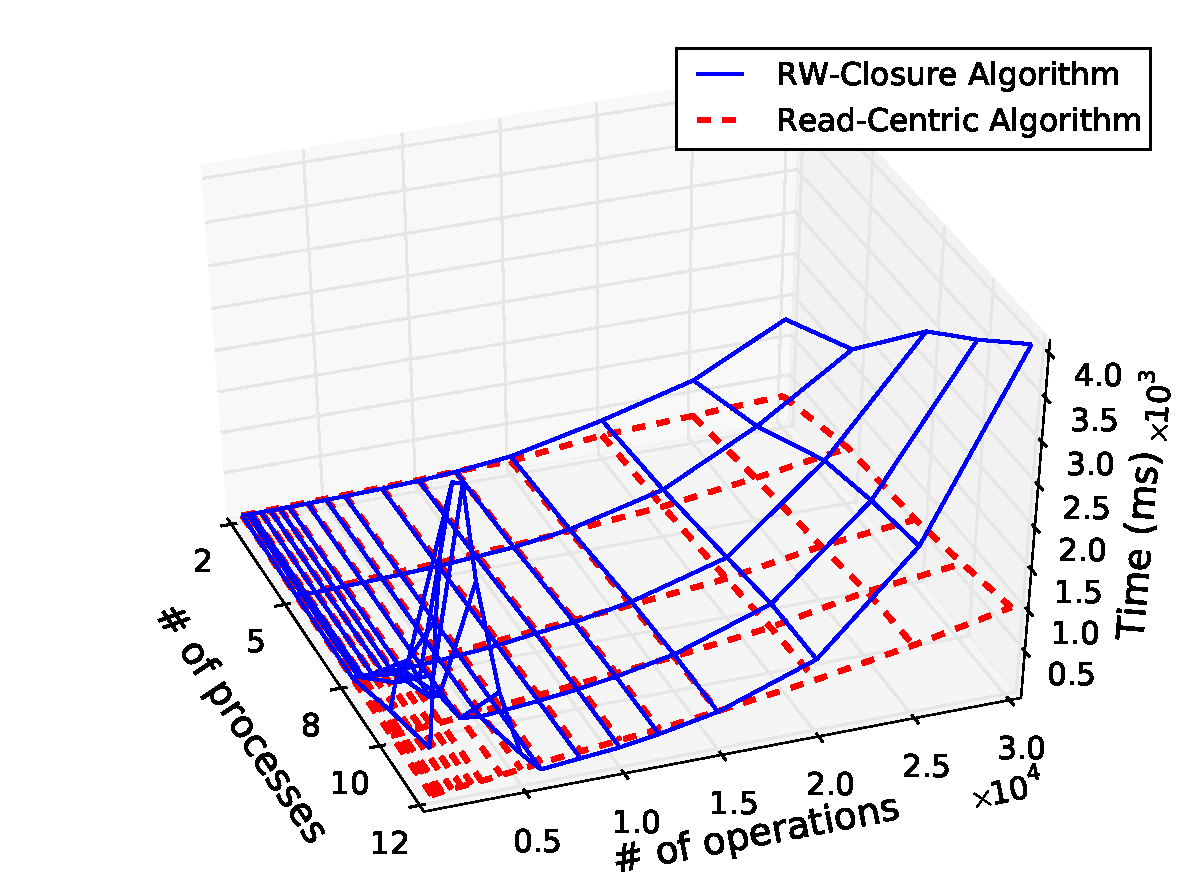
\includegraphics[width = 0.80\textwidth]{figures/vpc-random-cmp.pdf}
	\end{subfigure}%
	~
	\begin{subfigure}[t]{0.50\textwidth}
	  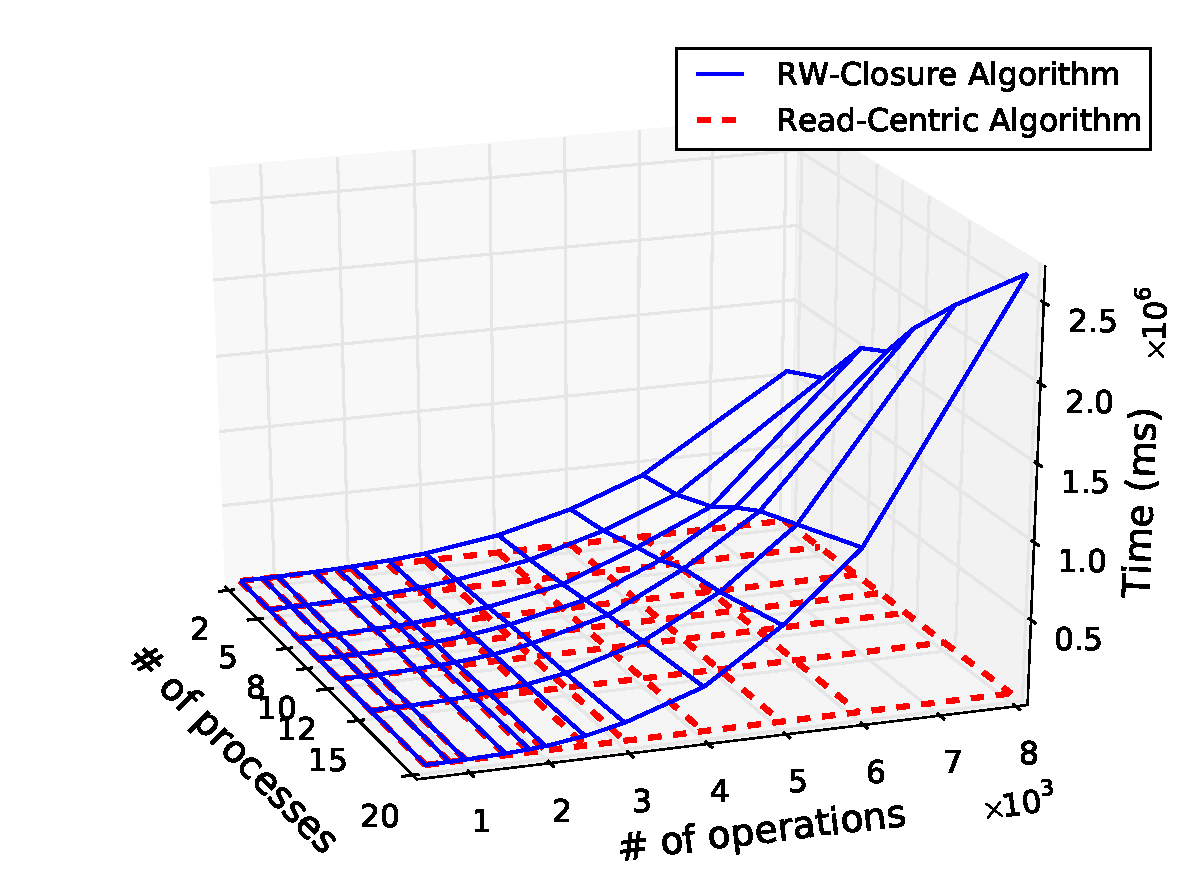
\includegraphics[width = 0.80\textwidth]{figures/vpc-valid-cmp.pdf}
	\end{subfigure}
	\caption{\rwclosure{} 算法与 \readcentric{} 算法在
	\textcolor{blue!80}{ (左) 随机生成}的执行及
	\textcolor{red!80}{ (右) 满足 \PRAM{} 一致性}的执行上的运行时间。}
  \end{figure}

  \pause
  \begin{center}
	\textcolor{red}{(右)} 20个进程、8,000 个操作: 

	\readcentric{} 可获得 694 倍加速.
  \end{center}
\end{frame}
%%%%%%%%%%%%%%%
\begin{frame}{实验评估}
  \fig{width = 0.45\textwidth}{figures/vpc-scalability-more.pdf}
  {\readcentric{} 算法在满足 \PRAM{} 一致性的执行上的运行时间.}

  \vspace{-0.30cm}

  \begin{description}
	\centering
	\item[\readcentric{}:] 20个进程、60,000个操作 < 600s~\footnotemark[1]~\footnotetext[1]{用于测试, 规模可用.}
	\item[\rwclosure{}:] 20个进程、8,000个操作 > 3,000s
  \end{description}
\end{frame}
%%%%%%%%%%%%%%%
\begin{frame}{VPC 的意义}
  \mdf{red}{blue}{对 VPC 问题的系统研究}{
	\begin{enumerate}
	  \item \readcentric{} 算法可用于测试系统是否正确实现了 \PRAM{} 一致性模型
	  \item \npcn{} 结果有助于理解弱一致性模型的复杂度
	\end{enumerate}
  }

  \pause
  \vspace{0.30cm}

  \mdf{red}{blue}{VPC 在相关工作中的意义}{
	较早关注 {\small (分布式系统领域)} ``弱一致性模型验证''问题 {\small (\textcolor{red}{2013$\sim$})}:
	\begin{description}
	  \item[强一致性:] \citeinbeamer{Gibbons}{SICOMP}{97} \citeinbeamer{Cantin}{TPDS}{05} \citeinbeamer{Golab}{PODC}{11} 
	  \item[弱一致性:] \citeinbeamer{Furbach}{ACSD}{14} \citeinbeamer{Bouajjani}{arXiv}{16}
	\end{description}
  }
\end{frame}
%%%%%%%%%%%%%%%
